\chapter{Titolo del secondo capitolo}
\label{chap:cap2}

Le assunzioni secondo cui ogni individuo possa entrare in contatto con chiunque (mixing omogeneo) e il numero di interazioni di ciascun soggetto sia confrontabile con quello degli altri non sono realistiche: anzi, la probabilità che si verifichi un incontro fra due individui presi a caso è praticamente infinitesima. Di norma, ognuno ha una serie di contatti regolari con un numero ristretto di persone (familiari, colleghi, etc), mentre ignora tutto il resto della popolazione; questo li rende particolarmente adatti ad essere rappresentati tramite una rete.
\medskip 
Andiamo ad introdurre una serie di definizioni che in seguito ci risulteranno utili. \\
\begin{definizione}[\textit{Grafo}]
Un \emph{grafo} (o una \emph{rete}) è un insieme di elementi detti vertici o \emph{nodi} che possono essere collegati fra loro da segmenti detti archi o \emph{link}.
\end{definizione}
\begin{figure}
		\begin{center}
			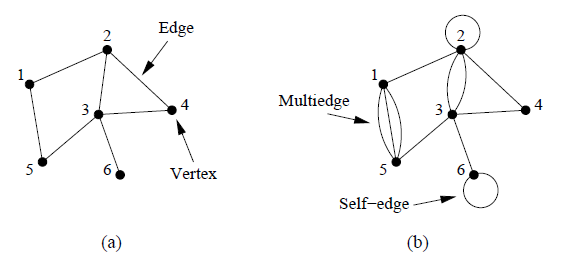
\includegraphics[scale=.8, keepaspectratio]{network_example}
			\caption{(a) Un grafo semplice, cioè privo di loop o link multipli. (b) Un grafo che presenta entrambi. \cite{Newman}}
			\label{fig:net_ex}
		\end{center}
	\end{figure}
	
Consideriamo una rete non orientata - cioè una rete in cui i link possono essere percorsi indistintamente in un verso e nell'altro - con $ n $ vertici, che andiamo ad etichettare da $ 1 \cdots a n $. Se indichiamo con $ \left( i, j \right) $ l'arco fra i nodi $ i $ e $ j $, allora l'intera rete può essere descritta in funzione della
\begin{definizione}[\textit{Matrice di adiacenza 1}]
La matrice di adiacenza \textbf{A} relativa ad un grafo non orientato è una matrice i cui elementi sono così definiti:
\[
A_{ij} \, =
\begin{cases}
1, & \text{se c'è un arco fra $ i $ e $ j $}\\
0, & \text{altrimenti}
\end{cases}
\]
\end{definizione}